\section{Optical Chain Development}

The system needs to be able to preform high resolution images of the atmosphere using the AOTF as the internal filter. It is an ideal device for space applications since it has no movable parts and a fast RF stabilization time; however, the AOTF limits the optical system to only have two functional layouts since the incoming light must enter the device at less than the acceptance angle. This is the maximum angle light can enter the device and still undergo the diffraction interaction. These two layouts are a telecentric and a telescopic system and will discussed in the following two sections. After, a section about the final decision for ALI will under took with rationalization on why the final design was chosen and a comparison to the Belgium instrument ALTIUS.

%The telescope or afocal system causes a wavelength gradient to be formed across the field of view of the image whereas the telecentric design overcomes this problem but has a larger FWHM \citep{Suhre2004} Currently Atmospheric Limb Tracker for the Investigation of the Upcoming Stratosphere (ATLIUS), a Belgium instrument, is being designed with an AOTF in a telecentric layout to remove the spectral gradient \citep{Dekemper2012}. However, the telecentric confocal system has a burring issue that must be corrected before it can be used in atmospheric spectroscopy.

\subsection{Telecentric System Prototype}
\label{sec:3.2:telecentricSystem}

The first system in consideration is a telecentric system. In order to describe the concept behind the telecentric system a basic ray tracing image is shown in \autoref{fig:3.2:rayTracing} where the three paraxial rays are drawn using a simple biconvex lens. %All the rays start from the top of the object and each travel in a certain path. The first ray called the parallel ray travel along the optical axis until it hits the refractive surface then passes through the focal point on the other side of the lens denoted by $f$. The second ray is called the focal ray and it passes through the object (left) side focal point and then travels parallel to the optical axis once it has interacted with the lens. And third the chief ray travels straight thought the center of the lens. These three rays all intersect on the image (right) side and show the location of the formed image.

\begin{figure}[h!]
    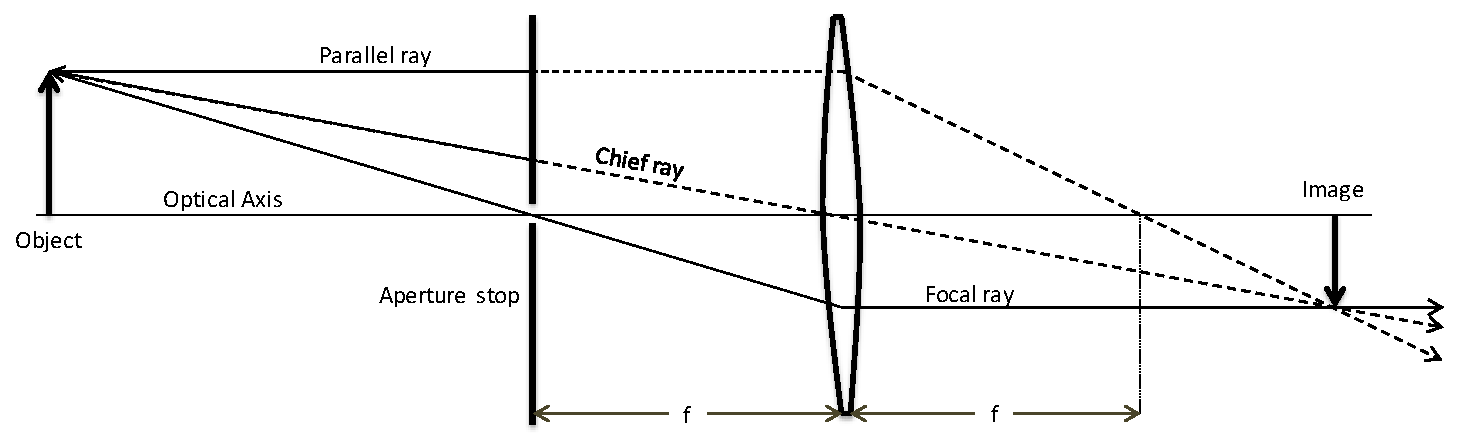
\includegraphics[width=1.0\textwidth]{./Images/3-2-RayTracing.pdf}
    \caption[Telecentric Ray Tracing Diagram]{A standard paraxial ray tracing diagram. The aperture is located to make the system telecentric in the image plane. $f$ is the focal length of the lens.}
    \label{fig:3.2:rayTracing}
\end{figure}

To make this ray tracing system telecentric in image space an aperture is added to the system on the object side at the focal point of the lens. The theoretical idea is to have an aperture so small that only the focal ray can pass through it. All of the other rays, including the chief and parallel ray, are blocked from entering the system. Now the image is only defined by a single ray and it is in focus everywhere on the image side of the system, and therefore has an infinite depth of field. However, a aperture that is so small proposes a few problems in practice. First, a hole of such a small size would cause diffraction effects that would dominate the imaging qualities of the system. Second, such a small aperture would let so little signal through that very long exposure times would be needed or a low signal to noise ratio would result. So in practice a larger aperture is used at the focal point. Now the system no longer has an infinite depth of field, but still retains a large value and the image still remains almost same size no matter where the image plane is located. It should be noted that a telecentric system in object space can be created by putting the aperture on the image side of the lens causing the the object to always be the same size in the image no matter where it is physically located.

%first it would be impossible to make a aperture that is small and is infinitely thin, and

A telecentric layout in both image and object space has an advantage for the imaging quality of the AOTF system shown in \autoref{fig:3.2:telecentricRayTracing}. Since the wavelength filtered by the AOTF is dependant on the incident angle, and from \autoref{fig:3.2:telecentricRayTracing}, all the lines of sight enter with approximately the same angular spread so the filtered image has consistent wavelength. However, two problems are added to the system. First, a blurring effect is added to the final image dependant on wavelength, which will be discussed below in greater detail. As well, this method is sensitive to any surface defects of the crystal since the light enters the crystal in focused bundles.

\begin{figure}[h!]
    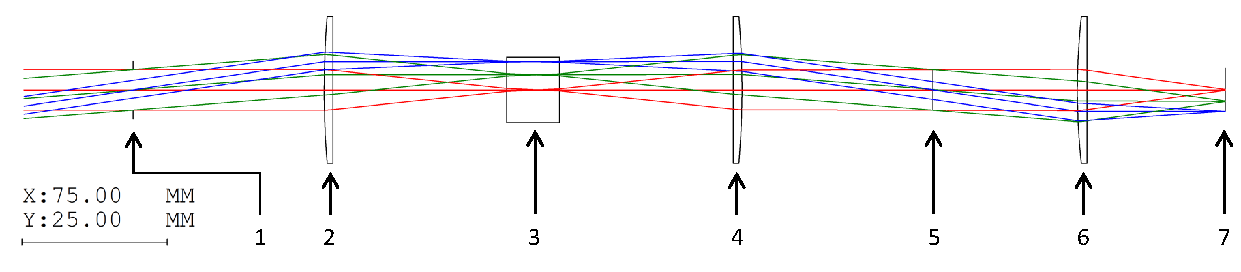
\includegraphics[width=1.0\textwidth]{./Images/3-2-TelecentricRayTracing.pdf}
    \caption[ALI Telecentric Design Prototype]{Ray Tracing diagram simulation of the telecentric lens system preformed using CODE V. The elements in the system are the following: (1) Optical Stop and telecentric aperture. (2) 100~mm focal length plano-convex lens. (3) Brimrose AOTF characterized in \autoref{sec:3.1:AOTFCalibration}. (4) 100~mm focal length plano-convex lens. (5) Telecentric Aperture. (6) 75.6~mm focal length plano-convex lens. (7) Imaging plane. It should be noted that the x and y scales are not the same in this image. Also, in the lab a polarizer is added in front and behind the AOTF as well as prisms after the AOTF.}
    \label{fig:3.2:telecentricRayTracing}
\end{figure}

As a part of this work a test optical system was designed to be telecentric in both object and image space with back end optics to resize the image to fit on the CCD. A list of the specifications can be seen in \autoref{tab:3.2:telecenticSystemParameters} and a ray tracing diagram from a Code V simulation is shown in \autoref{fig:3.2:telecentricRayTracing}. The AOTF has a optical aperture of 10~mm by 10~mm and is the system's field stop. This is a physical limit of the device and causes the field of view to be limited. In order to have lines of sight from the ground to the maximum float altitude of a stratospheric balloon, typically 35~km, a 6\si{\degree} field of view is required. Also with the current set up of 100~mm focal length lenses the rays of light from each line of sight enter the AOTF at the maximum acceptance angle, which is 4\si{\degree}. The acceptance angle is the maximum angle that light can enter the AOTF front aperture and still undergo Bragg diffraction. This allows the maximum amount of light to enter the device and recover the highest throughput as possible.

%However, the aperture of the AOTF limits the system to 5.7 degrees so assuming a 35 km balloon altitude the top kilometer will not be captured by the CCD. In reality this is a negligible loss since the line of sight looking out straight, directly tangential to the earth below, is viewing the least amount of atmosphere compared to any other line of sight, and as such, is not as information dense as lower lines of sight.

\begin{table}[h!]
    \begin{center}
    \begin{tabular}{|l|c|}
    \hline
    Effective focal length (mm) & 75.6 \\
    \hline
    Front optics focal length (mm) & 100 \\
    \hline
    Back optics focal length (mm) & 75.6 \\
    \hline
    Front optics magnification & 1.00 \\
    \hline
    Back optics magnification & 0.756 \\
    \hline
    Field of view ($^{\circ}$) & 5.7 x 5.7 \\
    \hline
    f-number & 14.28 \\
    \hline
    \end{tabular}
    \end{center}
    \caption{Telecentric System Optical Parameters.}
    \label{tab:3.2:telecenticSystemParameters}
\end{table}

The light is focused on a 16-bit digital QSI 616 CCD with a mechanical shutter that allows an integration time between 0.01~seconds to 240~minutes. The CCD chip itself is a Kodak KAF-1603ME with micro lenses to improve the quantum efficiently of the device and its spectral characteristics can be seen in \autoref{fig:3.2:QSIQuantumEfficientcy}.

\begin{figure}[h!]
    \begin{center}
    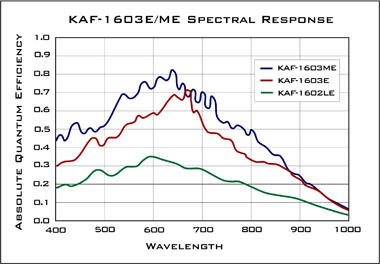
\includegraphics[width=0.5\textwidth]{./Images/3-2-QsiCcdQe.jpg}
    \caption[QSI 616 Camera Quantum Efficiency]{Quantum efficiency of the Kodak KAF-1603ME contained within the QSI CCD camera is represented by blue curve. Quantum efficiency provided by QSI Scientific. }
    \label{fig:3.2:QSIQuantumEfficientcy}
    \end{center}
\end{figure}

The overall design has several aspects that make it a good system for imaging. First all of the bundles of light entering the AOTF have the same angular spread. As seen in equation \autoref{eqn:3.1:AOTFWavelengthDependance} the diffracted wavelength depends on the incoming angle or its spread, in this set up all points of the imaging plane will have the same angular dependance so the entire image will be of the same wavelength and have the same spectral bandpass.

%Also, since the system is telecentric, perspective is not a major factor in the final image of the system as an object of same size but at different distances will appear to be the same size in the recorded image.

However, despite its benefits there are a few drawbacks to consider in the design as well. First, the optical path between the two 100~mm focal length lens is 200~mm in air, however the AOTF is made of TeO$_{2}$  or paratellurite and has a high index of refraction of 2.43 and 2.27 for the extraordinary and ordinary optical axis respectively. The crystal also has a high dispersive property, or Abbe number, so the index of refraction depends on the wavelength. The change is distance in the optical path, $d$, is given by
\begin{equation}
    \ d = \frac{n(\lambda)-1}{n(\lambda)}t
    \label{eqn:3.2:opticalPathDisplacement}
\end{equation}
where $n(\lambda)$ is the index of refraction with a wavelength dependance and $t$ is the thickness of the crystal. The AOTF crystal causes the optical path in air to be lengthened by $d$, as can be seen in \autoref{fig:3.2:opticalPathDisplacement}. In order to compensate, the length $d$ must be added to the path to account to the discrepancy, but this can only be accounted for a specific wavelength and thus image defocusing will occur at the image plane for other wavelengths. The severity of this problem can be seen in \autoref{fig:3.2:telecentricSpotSize} from a Code V simulation of the spot size of the optical system . In this simulation a grid of rays is passed through the system for each field of view and using ray tracing the final locations on the image plane are determined. The black circles represent the Airy disks, which are the minimum possible spot size possible limited by diffraction for each wavelength of light. The above analysis was preformed when the system was focused at 800~nm. The spot sizes at 800~nm are on the order of 24~\si{\micro\meter} at the center, which is diffraction limited, and 94~\si{\micro\meter} at the edge of the field of view. However, for the same optical layout the 600\,nm spot sizes are all greater than 160~\si{\micro\meter} which will cause an noticeable blurring in the recorded image.

\begin{figure}[h!]
    \begin{center}
    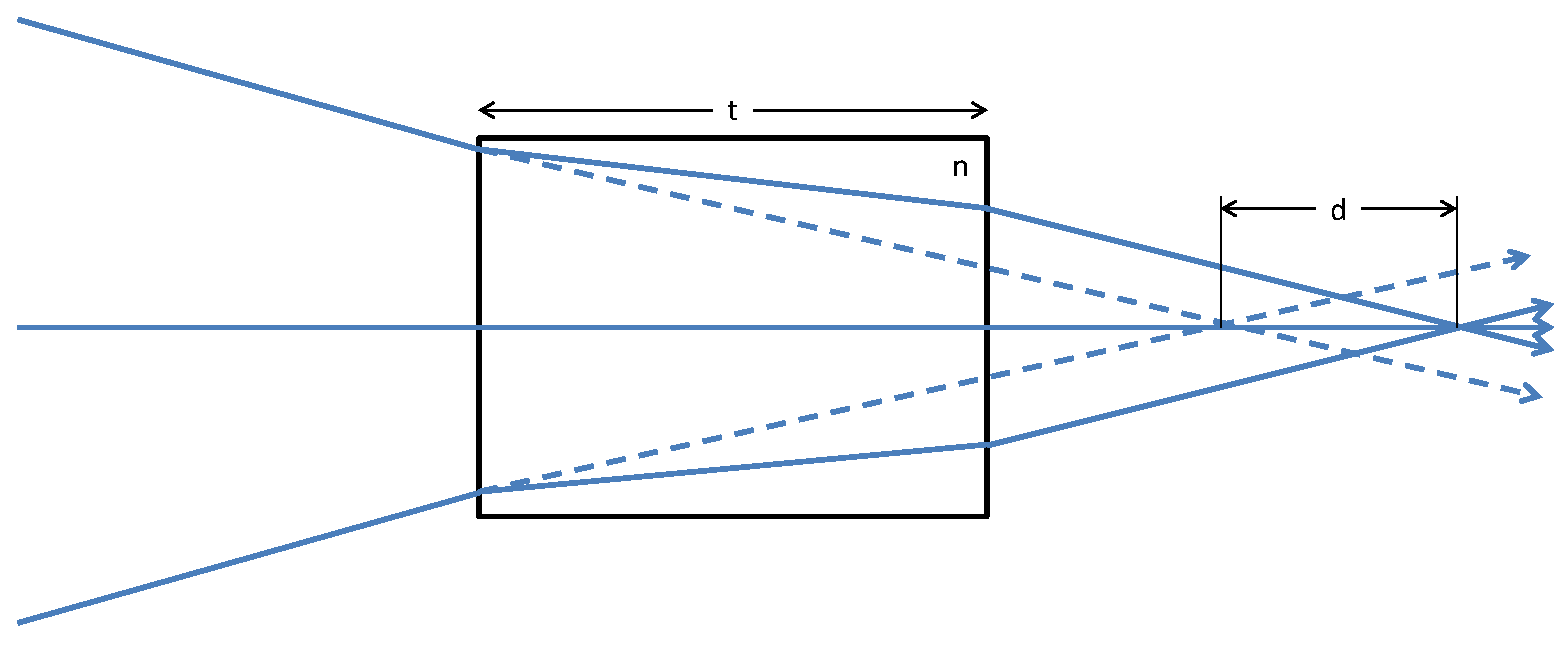
\includegraphics[width=1.0\textwidth]{./Images/3-2-OpticalPathDisplacement.pdf}
    \caption[Telecentric Optical Path Displacement]{The effect on the optical path of converging light bundles as they pass through an material of index of refraction $n(\lambda)$. When the index of refraction strongly depends on wavelength, as in the AOTF, the optical path length can expense great changes that will alter the focal point of the system.}
    \label{fig:3.2:opticalPathDisplacement}
    \end{center}
\end{figure}

\begin{figure}[h!]
    \begin{center}
    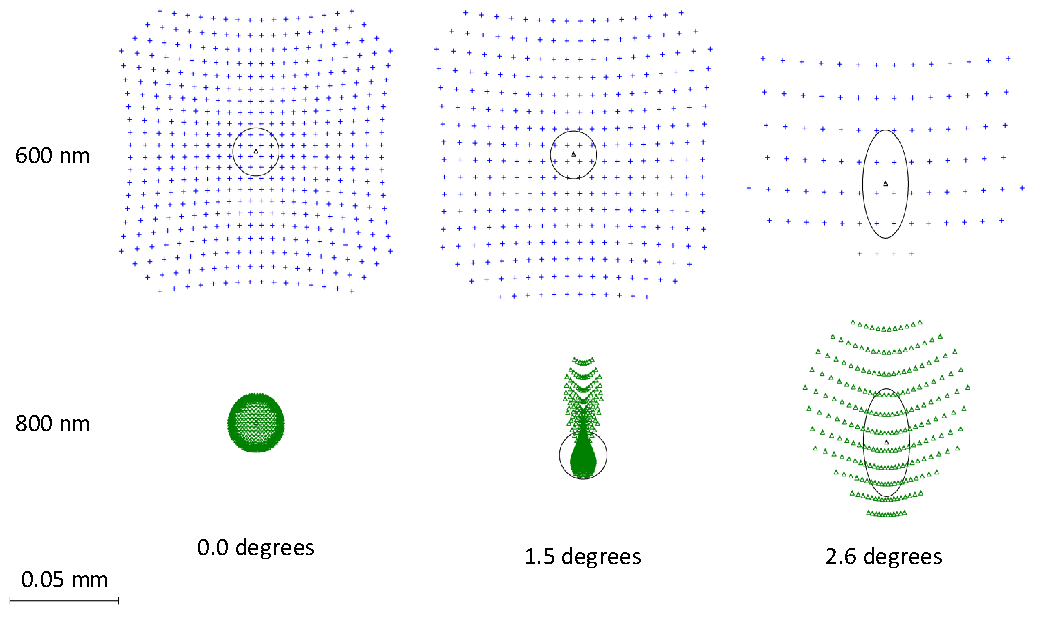
\includegraphics[width=1.0\textwidth]{./Images/3-2-TelecentricSpotSize.pdf}
    \caption[Telecentric Prototype Spot Sizes]{Code V simulation of the spot size for the telecentric system at focus at 800~nm. The spots are shown for 0.0, 1.5 and 2.6 degree fields of view at 600~nm (blue) and 800~nm (green). The full spot sizes for the 600~nm spots are 0.16, 0.22, and 0.25~mm for 0.0, 1.5, and 2.6\si{\degree} fields respectively, with the corresponding 800~nm spot sizes being 0.024, 0.053, 0.094~mm. The black circles represent the Airy disk for each specific wavelength and field of view.}
    \label{fig:3.2:telecentricSpotSize}
    \end{center}
\end{figure}

The system was bread boarded in the lab and used to image EIA 1956 standard resolution chart. The results of the test can be seen in \autoref{fig:3.2:telecentricTestImages}. The experimental set up is similar to the system in \autoref{fig:3.2:telecentricRayTracing} except for two fundamental differences. The Code V software can preform analysis for only one polarization and neglects the bend in the optical axis caused by the AOTF. However, these two issues can be dealt with sufficiently in the lab. The polarization issue is removed by added a polarizer before and after the AOTF. The light that is actively diffracted through the AOTF is the light that enters the AOTF crystal on the extraordinary polarization. The polarizer before the device stops the ordinary polarization from entering the device. The second polarizer on the other side of the device is used to only let the diffracted light through and removes the non-diffracted extraordinary polarization light. The interaction with the crystal causes the diffracted beam to be rotated by 90\si{\degree}, so the polarizers are rotated by 90 degrees with respect to each other. The second issue to be handled is that the AOTF bends the optical path by 2.7\si{\degree}. Two prisms were added after the ATOF to straighten out the optical path; the optical path past the prisms is parallel to the original optical path and is offset by approximately a millimeter and clips a part of the field of the view. The optical layout around the AOTF is similar to the optics around the AOTF in the characterization test shown in \autoref{fig:3.1:testExperimentalSetup}. The resolution chart was positioned so that the loss of the field of the view due to the prism compensation was accounted by a shift in the vertical location of the resolution chart since it only fills the whole field of view in the horizontal direction.

\begin{figure}[h!]
    \begin{center}
    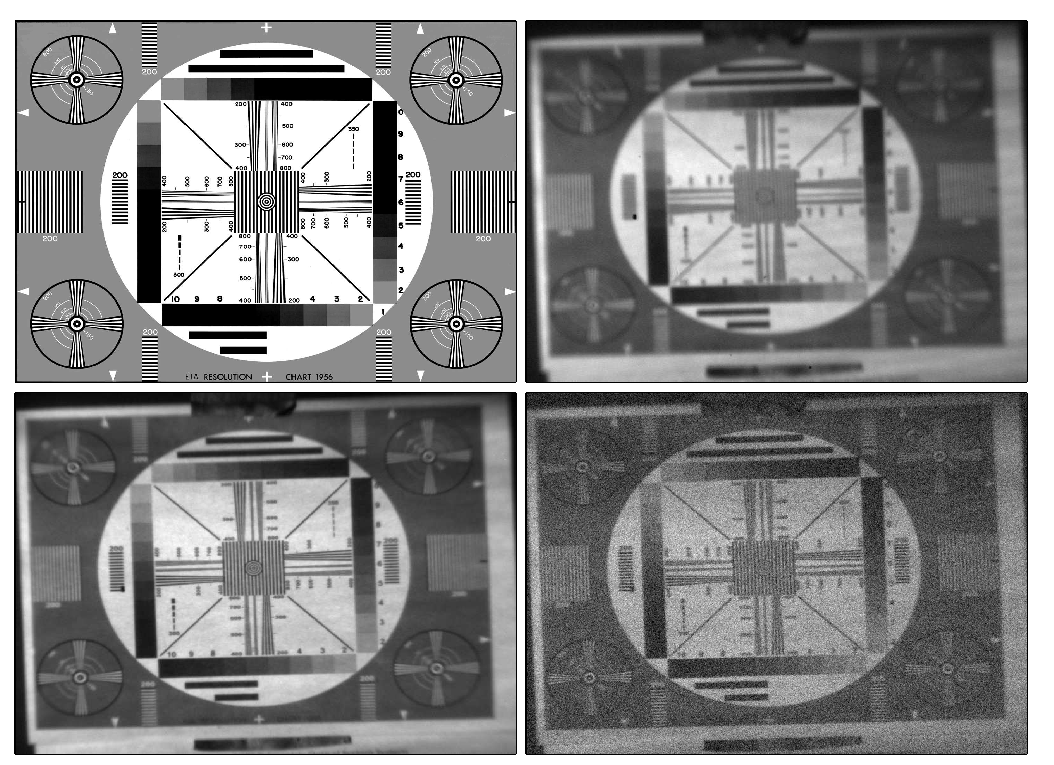
\includegraphics[width=1.0\textwidth]{./Images/3-2-TelecentricTestImages.pdf}
    \caption[Telecentric Prototype Laboratory Test Images]{The top left is the original test image used for the experiment. The top right, bottom left, and bottom right are the images recorded through the telecentric system at 650, 750, and 850~nm. The system is focused at 800~nm.}
    \label{fig:3.2:telecentricTestImages}
    \end{center}
\end{figure}

The images were taken using a 30 second exposures on the QSI CCD for each wavelength with the stray light, dark current, and DC offset removed from the image. From \autoref{fig:3.2:telecentricTestImages} the image blurring that was simulated in the spot size diagram can be easily noticed in the 650~nm wavelength image. The center lines of the resolution chart are unable to be resolved from each other compared to the 750~nm image. A unique line of sight can be resolved every 2 pixels in the center of the 750~nm image which corresponds to 150\,m resolution at the tangent point from the balloon platform, and a 3-4 pixel resolution near the edge corresponding to about a 200~m resolution. Also due to the efficiencies of the CCD the signal to noise ratio at the 850~nm image in the bottom right panel is rather low, and can be visibly seen by looking at the grainy quality of the image and will need to be addressed for the final device. Methods to resolved both of the above issues will be discussed in the future work section.

\subsection{Telescopic System Prototype}

The second optical system in consideration is a telescopic optical system consisting of a standard telescope with a focusing lens at the back end of the optical system. A simple astronomical telescope. The front lens, known as the objective lens, is used to focus an object at infinity to the focal point of the lens, then a second lens, the eyepiece is used to increase the optical power of the system, that is to increase the angular size of the image with respect to the angular size of the object. The eyepiece lens is located at a combined distance of the of the focal lengths of both the objective and eyepiece and causes the image to be focused at infinity. However for our system the telescope is used to focus the light in order to enter the AOTF at an angle less than its acceptance angle as well as to reject light rays outside of our field of view. The light from each line of sight in the telescopic system enters the AOTF collimated and is focused though a focusing lens onto the the QSI CCD discussed in section \autoref{sec:3.2:telecentricSystem}. A detailed simulated Code V layout of the optical design can be seen in \autoref{fig:3.2:telescopicRayTracing}.

%The magnification is given by

%\begin{equation}
%    \ M_{\theta} = -\frac{f_{o}}{f_{e}}
%    \label{eqn:telescopeMagnification}
%\end{equation}

%where $M_{\theta}$ is the optical power or the angular magnification, and $f_{o}$ and $f_{e}$ are the focal lengths of the objective and eyepiece respectively.

\begin{figure}[h!]
    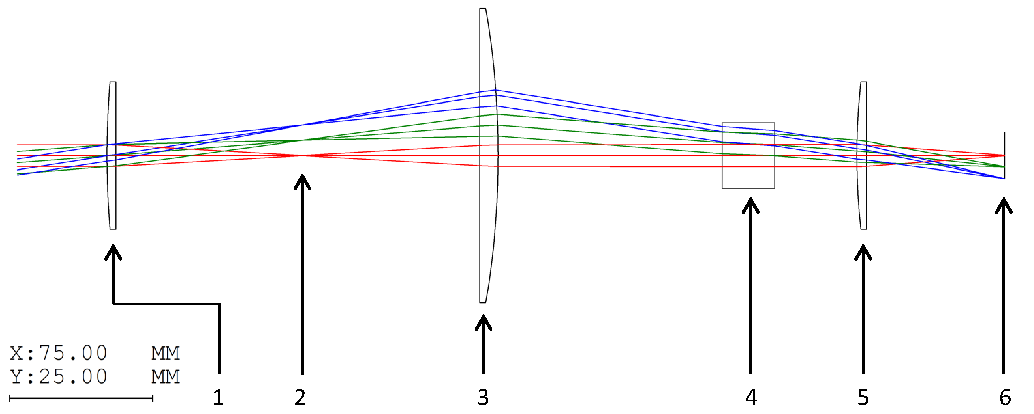
\includegraphics[width=1.0\textwidth]{./Images/3-2-TelescopicRayTracing.pdf}
    \caption[ALI Telescopic Design Prototype]{Ray Tracing diagram of the telescopic lens system simulated by Code V. The elements in the system are the following: (1) 100~mm focal length plano-convex lens. (2) Location where shutter will be located to limit stray light (3) 100~mm focal length plano-convex lens. (4) Brimrose AOTF characterized in \autoref{sec:3.1:AOTFCalibration}. (5) 75.6~mm focal length plano-convex lens. (6) Imaging plane. It should be noted that the x and y scales are not the same in this image. Also, in the lab a polarizer is added in front and behind the AOTF as well as prisms behind the AOTF.}
    \label{fig:3.2:telescopicRayTracing}
\end{figure}

This system was designed with as many similar components as possible to the telecentric system in order to allow comparisons of the system to be made without major optical effects and abberations caused by using different materials, sizes, and focal length lens. The optical specifications of this system are given in \autoref{tab:3.2:telescopicSystemParameters}. However, there are fundamental differences, the aperture stop is located at the front lens which limits the rays of light that can enter the system, unlike the telecentric design that has a front aperture at the focal length of the first lens.

%Therefore, this system has perspective in the final image, meaning objects further away look smaller in the final image.

\begin{table}[h!]
    \begin{center}
    \begin{tabular}{|l|c|}
    \hline
    Effective focal length (mm) & 75.6 \\
    \hline
    Front optics focal length (mm) & 100 \\
    \hline
    Back optics focal length (mm) & 75.6 \\
    \hline
    Front optics magnification & 1.00 \\
    \hline
    Back optics magnification & 0.756 \\
    \hline
    Field of view ($^{\circ}$) & 6.0 x 6.0 \\
    \hline
    f-number & 20 \\
    \hline
    \end{tabular}
    \end{center}
    \caption{Telescoptic System Optical Parameters.}
    \label{tab:3.2:telescopicSystemParameters}
\end{table}

The AOTF now has collimated light passing though the device, unlike the telecentric system, and this has a few fundamental changes to alter to the system's imaging quality. First, the primary light passing through the AOTF from a single line of sight is entering the AOTF at the same angle, so the image will have a smaller FWHM than the telecentric counterpart however each line of sight will be diffracted with a different fundamental wavelength due to the angular dependance in the AOTF Bragg diffraction wavelength determination equation (\autoref{eqn:3.1:AOTFWavelengthDependance}). The final image has a smaller spectral bandpass but there will a wavelength gradient radiating out from the center of the image. Second, since the light now passes through the AOTF collimated, the focal point of the image no longer changes with wavelength. Instead a lateral displacement of each line of sight occurs based on the angle of incidence and the diffracted wavelength which causes a slight magnification of the image. The lateral displacement that occurs is given by the following relation
\begin{equation}
    \ \delta = (n(\lambda)-1)\frac{t\theta}{n(\lambda)}
    \label{eqn:3.2:planeParallelDiplacement}
\end{equation}
where $\delta$ is the displacement from the original path; causing a slight magnification change based on the wavelength of the light being diffracted, but this magnification is a negligible change overall, the effect can be seen in \autoref{fig:3.2:planeParallelDiplacement}. The last change to the system is the focusing power it possesses, as can be seen in the spot diagrams in \autoref{fig:3.2:telescopicSpotSize}. The change in spot size due to wavelength is primarily due to the chromatic aberrations of the optical lens. One option is to replace the lenses with mirrors in the flight version which will eliminate the chromatic abberation issue. Second, the system is diffraction limited for 600\,nm for all lines of sight and at 800\,nm at 3.0 degrees. Also the difference in location of the spot sizes is caused by the magnification effect discussed above.

\begin{figure}[h!]
    \begin{center}
    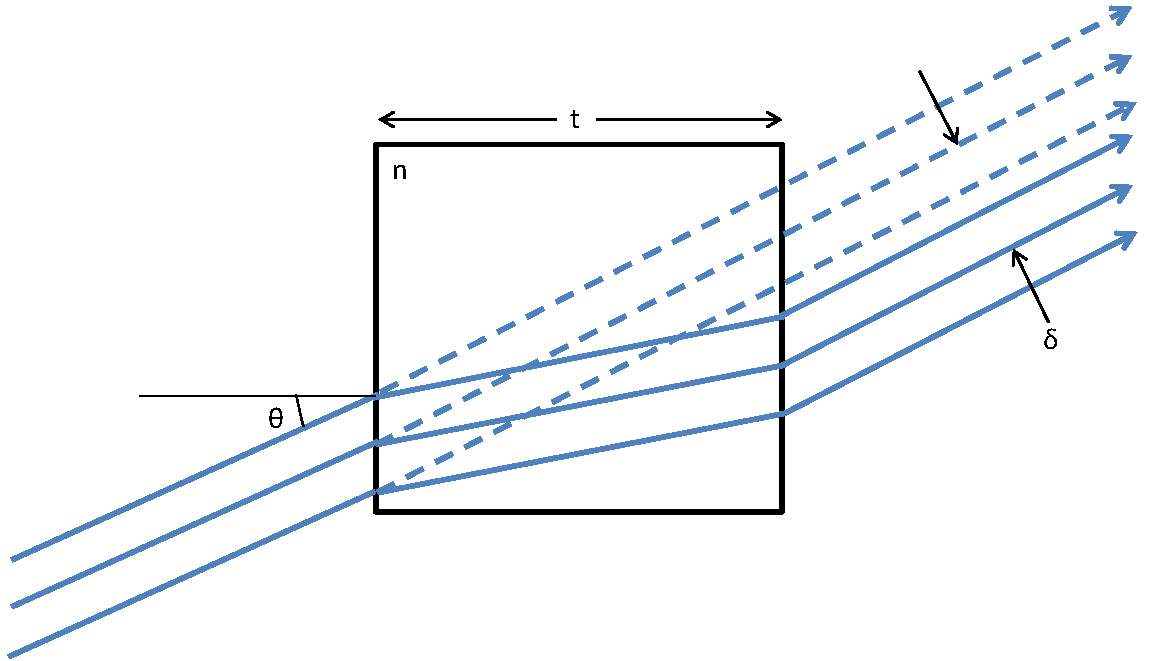
\includegraphics[width=1.0\textwidth]{./Images/3-2-PlaneParallelDisplacement.pdf}
    \caption[Telescoptic Plane Parallel Displacement]{Vertical displacement of a collimated bundle of light cause by a material of index of refraction $n$.}
    \label{fig:3.2:planeParallelDiplacement}
    \end{center}
\end{figure}

\begin{figure}[!h]
    \begin{center}
    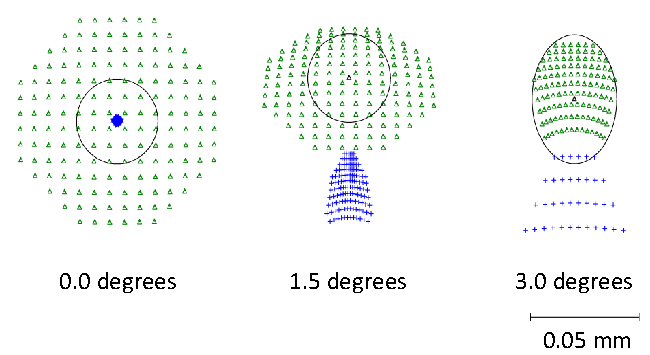
\includegraphics[width=0.70\textwidth]{./Images/3-2-TelescopicSpotSize.pdf}
    \caption[Telescopic Prototype Spot Sizes]{Code V simulation of the spot size for the telescopic system. The spots are shown for 0.0, 1.5 and 3.0\si{\degree} fields of view at 600~nm (blue) and 800~nm (green). The full spot sizes for the 600~nm spots are 0.004, 0.045, and 0.122~mm for 0.0, 1.5, and 3.0\si{\degree} fields respectively, with the corresponding 800~nm spot sizes being 0.096, 0.081, 0.047~mm. The black circles represent the Airy disk for each specific wavelength and field of view.}
    \label{fig:3.2:telescopicSpotSize}
    \end{center}
\end{figure}

An experimental resolution test was set up similar to the one described in \autoref{tab:3.2:telecenticSystemParameters} with two polarizers and prisms added to the optical chain. The QSI CCD was also used with the same 30 second integration time. The results of this test can be seen in \autoref{fig:3.2:telescopicTestImages}. Once again the image at 750~nm is the sharpest of the three but the center lines of the EIA 1956 test chart are distinguishable at all of the wavelengths. The blurring of the 650~nm image is caused by the chromatic abberations of the lens and the prisms and will removed if mirrors are used in the final design. Also, the magnification issue discussed above is relatively insignificant in the test images and the small changes can be accounted for in the calibration of the final instrument. Lastly, the low NIR levels of the light source combined with the poor quantum efficiency of the CCD camera causes the 850~nm image to also have a low signal to noise ratio. This issue will have to be dealt with in the final design, which as mentioned may include an InGaAs sensor array. A final note to be made is the gradient found in the brightness of these images. This is currently thought to be a vignetting problem due to an optical misalignment and is under investigation.

\begin{figure}[h!]
    \begin{center}
    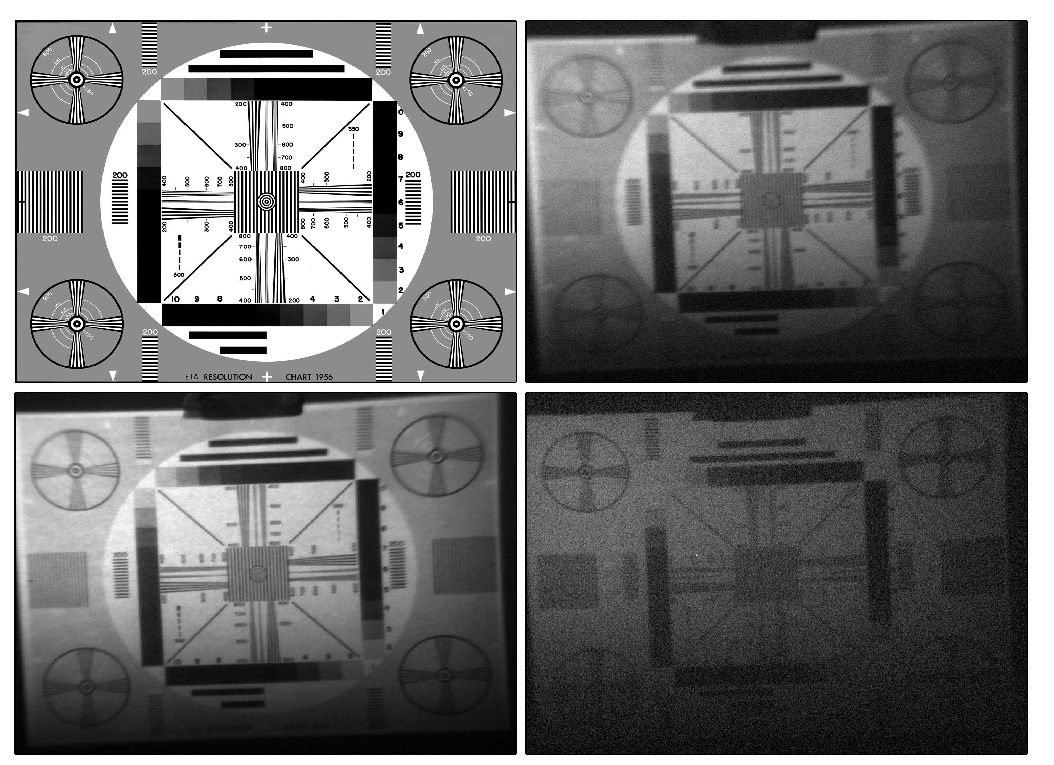
\includegraphics[width=1.0\textwidth]{./Images/3-2-TelescopicTestImages.pdf}
    \caption[Telescoptic Prototype Laboratory Test Images]{The top left is the original test image used for the experiment. The top right, bottom left, and bottom right are the images recorded through the telescopic system at 650, 750, and 850~nm. The system is focused at 800\,nm.}
   \label{fig:3.2:telescopicTestImages}
    \end{center}
\end{figure}

\subsection{Final Choice}

A final selection for the optical design of ALI will be presented in this section as well the justifications used to determine the result. Furthermore, a comparison with the prototype Belgium instrument will be made to demonstrate the differences between the two instruments. For the final design of ALI the telescopic system deemed to be the better option for our scientific purpose to determine aerosol extinction and engineering study to verify the capabilities of using an AOTF in space based remote sensing techniques.

The telescopic system offers the ability of having an image plane location that is not dependant of the wavelength being imaged leading to a system that would either require the system to have mechanical pieces to move the imaging plane or additional optical components to counter act the change in the optical path. Using mechanic components to move the camera would be an addition failure point and would have to be well calibrated across the whole wavelength range. For the other alternative a custom lens or prism would need to be created in order to counteract the defocusing effect of the AOTF which would cause further reflections within the system increasing the possibility of stray light hitting the CCD camera and well at decreasing the signal through put of the system. This design also allow for a greater focus on spacial resolution that could be achieved with a telescopic system with is necessary in order to be able to image the fine structure of aerosol concentration on the order of 100s of metres.

Another minor consideration for the system is the finer FWHM for each line of sight that passes through the ATOF and is imaged on the CCD giving more fine spectral resolution however the draw back is that the central wavelength of each line of sight is dependant upon the angle of incident. A wavelength gradient appears in the final image in the the longest central wavelength occurs in the center of the image and radiates outward towards shorter wavelengths as apparent in \autoref{eqn:3.1:AOTFWavelengthDependance} an have a wavelength gradient of approximately 7~nm at 650~nm central wavelength and 11~nm at 950~nm, however for a space based instrument with a relatively smaller field of view the gradient could be reduced to as small as 2~nm across the whole image with, at worse, the same size as the FWHM of the AOTF. The effect would be a significant problem for instruments measuring trace gasses absorbtion lines, for example water vapour, but aerosol is a broadband enhancing feature in which its effect are visible in atmospheric measurement from 400~nm well into the IR. The wavelength dependant magnification mentioned earlier only amounts to being a change of a approximately 4 pixels in both direction from the inherent magnification from 650~nm to 950~nm overall this change is considered negligible for the purpose of ali's mission which will be discussed in \autoref{sec??}.

The final optical specification for ALI can be found in \autoref{tab:3.2:ALISystemParameters}. A noticeable change from the telescopic prototype is the decreased f/\# and the front end demagnification and the back end magnification which have all were all related to increasing the signal entering ALI. The lower F/\# increases the amount of light that can enter the optical chain allowing for shorter exposure time that were needed in order to get high quality data from the Timmins, Ontario campaign. The increase F/\# required larger optics and has as such a larger beam of light to pass into the AOTF, which unfortunately was not possible due to the AOTF having a fixed aperture of 10 by 10~mm. To rectify this problem a found end demagnification was added to reduce the size of the incoming light beam entering he AOTF down to a size that could pass through its optical aperture and remagnify it back to its original size with the back end optics before passing into the imaging system. Lastly, the specifications for the wavelength range was decreased from 600-1200~nm down to 650-950~nm, which was done for two different reason at each end of the spectrum. At the 600~nm side of the range the effeminacy of the optical components antireflection coasting started to fall and the AOTF itself diffraction efficiency fall off quickly at wavelengths lowers than 630~nm. These loss in efficiencies would require large integration times during flight that would not have been practical so they were removed from the instruments range, and even 650~nm has exposure time on the longer side of reasonable. At the long wavelengths the system was originally have a beam splitter to have the image focused on an InGa array for the NIR and a CCD for the visible region which was to be implemented when a folded mirror optical system was to be implemented, but the launch date for ALI was pushed up by one year and no longer gave the time required to design the folded optical system so a linear lenses non-beam spitted system was to be used in stead. The inherent nature of the change of date made it a requirement to reduce upper limit of ALI's wavelength range to 950~nm instead of the originally proposed 1200~nm.

\begin{table}[!ht]
    \begin{center}
    \begin{tabular}{|l|c|}
      \hline
      Effective focal length (mm) & 74.3 \\
      \hline
      Front optics magnification & 0.67 \\
      \hline
      Back optics magnification & 1.27 \\
      \hline
      Field of view (\si{\degree}) & 6.0 x 6.0 \\
      \hline
      F-number & 7.5 \\
      \hline
      Image Size (mm) & 9x9\\
      \hline
      Spectral Range (nm) & 650-950\\
      \hline
    \end{tabular}
    \end{center}
    \caption{ALI Final System Optical Parameters.}
    \label{tab:3.2:ALISystemParameters}
\end{table}

 ALTIUS, a Belgium instrument, uses similar technology as ALI except uses a telecentric optical layout and is designed to measure atmospheric trace gases \citep{Dekemper2012}. Trace gases have narrow absorbtion to emission features that require specific wavelength knowledge. A telecentric layout will give a of constant wavelength across the whole field of view to be able to be able to resolve absorbtion features. The optical specifications are similar between the two instruments, however two key differences will be noted. First, the field of view of ALTIUS is smaller at 5.73x5.73\si{\degree} and if ALI would have used a telecentric design then it would have had an identical field of view due to the geometry and optical requirements of the telecentric layout. In a telecentric design the AOTF aperture directly limits your instruments field of view and both system use an ATOF crystal with an optical aperture of 10x10~mm. Second, the f-number for ALTIUS is 14.32 compared to ALI's 7.5 which allows ALI to increase light throughput at the cost of higher abberations in the final image.
